\documentclass[article]{jss}

%% -- LaTeX packages and custom commands ---------------------------------------

%% recommended packages
\usepackage{orcidlink,thumbpdf,lmodern,framed,float,amsmath}

%% new custom commands
\newcommand{\class}[1]{`\code{#1}'}
\newcommand{\fct}[1]{\code{#1()}}

%% For Sweave-based articles about R packages:
%% need no \usepackage{Sweave}



%% -- Article metainformation (author, title, ...) -----------------------------

%% - \author{} with primary affiliation (and optionally ORCID link)
%% - \Plainauthor{} without affiliations
%% - Separate authors by \And or \AND (in \author) or by comma (in \Plainauthor).
%% - \AND starts a new line, \And does not.
\author{Yanrong Song\\Columbia University
   \And Zijie Zhu\\Columbia University
   \And David Kane\\Harvard University
   \AND Ziqi Lu\\Harvard University
   \And Karan Tibrewal\\Williams Collage
   \And Fan Zhang\\Williams Collage}
   
\Plainauthor{Yanrong Song, Zijie Zhu, David Kane, Ziqi Lu, Karan Tibrewal, Fan Zhang}

%% - \title{} in title case
%% - \Plaintitle{} without LaTeX markup (if any)
%% - \Shorttitle{} with LaTeX markup (if any), used as running title
\title{Backtest Graphics in \proglang{R}}
\Plaintitle{Backtest Graphics in R}
\Shorttitle{Backtest Graphics in \proglang{R}}

%% - \Abstract{} almost as usual
\Abstract{
The \pkg{backtestGraphics} package provides an interactive graphical interface to visualize backtests results for a variety of financial instruments (equities, futures, credit default swaps, et cetera).The \pkg{Shiny} interface, returned by the package, contains a sidebar panel with summary and detailed performance statistics, such as number of instruments, cumulative and annualized profit and loss, Sharpe ratio, top three drawdowns, and the three best and worst performers in the backtest. The main panel of interface houses interactive plots of profit and loss (P\&L), net market value (NMV) and gross market value (GMV). Lastly, the package also supports vizualization of multiple strategies, sub-strategies, and overlapping portfolios that may be present in a single backtest result. 
}

%% - \Keywords{} with LaTeX markup, at least one required
%% - \Plainkeywords{} without LaTeX markup (if necessary)
%% - Should be comma-separated and in sentence case.
\Keywords{backtesting, vizualization, \proglang{R}}
\Plainkeywords{backtesting, vizualization, R}

%% - \Address{} of at least one author
%% - May contain multiple affiliations for each author
%%   (in extra lines, separated by \emph{and}\\).
%% - May contain multiple authors for the same affiliation
%%   (in the same first line, separated by comma).
\Address{
  Yanrong Song\\
  Columbia University in the City of New York\\
  Financial Engineering\\
  URL: \url{https://github.com/yanrong-stacy-song}
}



\begin{document}


%% -- Introduction -------------------------------------------------------------

%% - In principle "as usual".
%% - But should typically have some discussion of both _software_ and _methods_.
%% - Use \proglang{}, \pkg{}, and \code{} markup throughout the manuscript.
%% - If such markup is in (sub)section titles, a plain text version has to be
%%   added as well.
%% - All software mentioned should be properly \cite-d.
%% - All abbreviations should be introduced.
%% - Unless the expansions of abbreviations are proper names (like "Journal
%%   of Statistical Software" above) they should be in sentence case (like
%%   "generalized linear models" below).

\section[Introduction]{Introduction} \label{sec:intro}


Backtesting is the process of testing trading strategies on prior time horizons to measure the effectiveness of the given strategy. It helps investors understand and optimize their trading strategies [\cite{backtest}]. The \pkg{backtestGraphics} package provides an interactive \pkg{Shiny} interface to visualize backtest results for a variety of financial instruments (equities, futures, and credit defualt swaps, among others) [\cite{shiny}]. These visualizations enable users to employ their human perception to process a lot of backtest data quickly and approximately [\cite{bostock}].

\noindent
It is important to note here that \pkg{backtestGraphics} doesn't run backtests, but instead provides graphical visualization of backtest results. To illustrate this subtle distinction, consider a simple trading strategy that buys the top 10 shares of the S\&P 500, and shorts the bottom 10. Now, to test how the strategy performs historically, the user may use backtesting software like \emph{Quantopian}, or even  R packages like \pkg{backtest} [\cite{backtest}].The output from such backtesting is generally in the form of large data frames which are difficult to interpret. As of such, the user may feed these data frames, i.e. the holding data, to \pkg{backtestGraphics}. The package then constructs interactive \pkg{dygraph} plots, and calculates essential summary statistics which are easy to interpret and explore [\cite{dygraphs}].

\noindent
The \pkg{Shiny} interface returned by the package consists of a sidebar panel that includes a "Summary" and a "Detail" tab. The former provides the user with summary statistics, such as average gross market value (GMV), net market value (NMV), number of instruments, cumulative and annualized profit and loss (P\&L), Sharpe ratio and best and worst performing months. The "Detail" tab provides information about the best and worst performers, as well as the biggest drawdowns. 

\noindent
The main panel of the \pkg{Shiny} interface houses interactive plots for cumulative and point-in-time P\&L, NMV, GMV and number of contracts. The interactive nature of these plots provide the user with additional flexibility in exploring her backtest results by enabling her to zoom into specific time periods, or learn the value of a given response variable on a specific date.



\noindent
Additionally, to accomodate for more complex backtests, \pkg{backtestGraphics} allows the user to subset seamlessly between overlapping portfolios, and multiple strategies and sub-strategies. For example, suppose the user splits his portfolio into two halves: the first half trades using the aforementioned trading strategy on a weekly basis, while the second uses the same strategy on a bi-weekly basis. Although these strategies overlap every other week, the user may want to explore how a particular strategy does in isolation. In order to do so, the user simply has to select the appropriate options from the dropdown menus provided in the side bar panel.  



%% -- Manuscript ---------------------------------------------------------------

%% - In principle "as usual" again.
%% - When using equations (e.g., {equation}, {eqnarray}, {align}, etc.
%%   avoid empty lines before and after the equation (which would signal a new
%%   paragraph.
%% - When describing longer chunks of code that are _not_ meant for execution
%%   (e.g., a function synopsis or list of arguments), the environment {Code}
%%   is recommended. Alternatively, a plain {verbatim} can also be used.
%%   (For executed code see the next section.)

\section{Data} \label{sec:data}

The package comes with three sample data frames: \code{commodity}, \code{equity}, and \code{credit}. These are backtest results for commodity futures, equities, and credit default swaps (CDS), respectively. We use these data frames to demonstrate the capabilities of the backtestGraphics package. (Note: The user may also use her own data frame, as long as it adheres to the format specified in the documentation).

\subsection{Equity}

Let us begin with some details of \code{equity}. Equities are financial instruments that represent an ownership claim entitling the holder to dividends and ownership rights of the company for which the equities are issued [\cite{equities}].The \code{equity} data frame contains holding data for a trading strategy dealing with equities. 


\begin{Schunk}
\begin{Soutput}
 name       date sector       nmv        pnl
  A.Z 2005-05-02    MAT -131926.1  3158.4525
 ABFS 2005-05-02    IND -131926.1 -4058.6214
 ABS. 2005-05-02    CNS -131926.1  -733.2929
  A.Z 2005-05-03    MAT -128767.7  3644.3684
 ABFS 2005-05-03    IND -135984.7  -335.9721
 ABS. 2005-05-03    CNS -132659.4   733.2935
  A.Z 2005-05-04    MAT -125123.3 -1457.7478
 ABFS 2005-05-04    IND -136320.7 -1595.8684
 ABS. 2005-05-04    CNS -131926.1 -2466.5317
\end{Soutput}
\end{Schunk}

\begin{itemize}
\item{\code{name:} column contains the each stock's symbol.}
\item{\code{date:} column contains the trading date. (Note: this column must be of  \code{Date} type)}.
\item{\code{sector:} column contains the sector of each stock.}
\item{\code{nmv:} column contains the NMV at the beginning of the trading day for each stock. (Note: all values must be converted to the same currency). 
}
\item{\code{pnl:} column contains P\&L of each stock. (Note: all values must be converted to the same currency). 
}
\end{itemize}

\subsection{Commodity}

\noindent
Now, let us look at \code{commodity}. Simply put, a commodity futures contract is a legally binding agreement that provides for the delivery of the specified value of the said commodity at a specific time period in the future [\cite{futures}]. The \code{commodity} data frame consists of holding data from a trading strategy dealing in such commodity futures. 

\begin{Schunk}
\begin{Soutput}
          name id       date      sector portfolio   strategy
         brent CO 2003-02-03      energy         1 Strategy 1
         brent CO 2003-02-03      energy         6 Strategy 1
 cattle feeder FC 2003-02-03   livestock         1 Strategy 3
     cbt wheat  W 2003-02-03 agriculture         1 Strategy 3
     cbt wheat  W 2003-02-07 agriculture         1 Strategy 3
  substrategy      gmv    nmv      pnl contract
 Strategy 1.1   921600 921600 -21600.0       30
 Strategy 1.2   445440 445440 -10441.5       14
 Strategy 3.1 10426000 -58500  -7280.0      260
 Strategy 3.2  3616300  14500   5800.0      232
 Strategy 3.2  3738100  23200  23200.0      232
\end{Soutput}
\end{Schunk}

The columns \code{name}, \code{date}, \code{sector}, \code{nmv}, and \code{pnl} have the same meaning as the ones in \code{equity}. The remaining columns are listed below: (Note: these columns are optional). 

\begin{itemize}
\item{\code{ID:} column contains ID information for different commodities. }
\item{\code{strategy:} column contains the strategy number.
}
\item{\code{substrategy:} column contains the sub-strategy number.
}
\item{\code{gmv:} column contains the GMV of a given commodity at the start of each trading day  (Note: all values must be converted to the same currency). 
}

\item{\code{contract:} column contains the number of contracts of a given commodity at the start of each trading day.  
}
\end{itemize}

\subsection{Credit}

Finally, we look at \code{credit}. Credit Default Swaps (CDS) are a type of credit derivative that transfers the credit risk from one group of investors to another, in exchange for payment [\cite{CDS}]. The \code{credit} data frame contains holding data from a trading strategy dealing in such CDS. 

\begin{Schunk}
\begin{Soutput}
         name       date          sector  strategy   gmv      nmv
  AA.Senior.5 2008-10-01 Basic Materials     daily 9e+06 259259.3
  AA.Senior.5 2008-10-01 Basic Materials   monthly 9e+06 259259.3
  AA.Senior.5 2008-10-01 Basic Materials quarterly 9e+06 259259.3
 ABY.Senior.5 2008-10-01 Basic Materials     daily 9e+06 259259.3
 ABY.Senior.5 2008-10-01 Basic Materials   monthly 9e+06 259259.3
 ABY.Senior.5 2008-10-01 Basic Materials quarterly 9e+06 259259.3
  AA.Senior.5 2008-10-02 Basic Materials     daily 9e+06 170731.7
 ABY.Senior.5 2008-10-02 Basic Materials     daily 9e+06 170731.7
  AA.Senior.5 2008-10-03 Basic Materials     daily 9e+06 170731.7
 ABY.Senior.5 2008-10-03 Basic Materials     daily 9e+06 170731.7
          pnl
     570.9305
       0.0000
  -55605.8350
  -65521.3738
 1343776.6544
  356766.3732
   39295.1220
 -149936.6291
   75865.3799
  349670.0335
\end{Soutput}
\end{Schunk}

\noindent
Most of the columns here are the same as those in e\code{equity} and \code{commodity}. Notice that the \code{strategy} column here is used to denote backtest results for different trading frequencies. Towards this, the user must provide all backtest observations for each instrument, even when the position on the instrument is held and unchanged. This is because \pkg{backtestGraphics} uses the time gaps between each observation to determine the trading frequencies, and to calculate the annualized statistics. 



\section{Using the backtestGraphics Interface} \label{sec:backtestgraphics}

In this section, we discuss the functionality of various components of the \pkg{Shiny} interface returned by the \pkg{backtestGraphics} function. To use backtestGraphics, the user is required to pass in a data frame with \code{date}, \code{ID/name}, \code{NMV} and \code{P\&L} columns to the \pkg{backtestGraphics} function. Additionally, the user can also pass in optional columns, such as \code{sector}, \code{GMV}, \code{contracts}, \code{strategy}, \code{substrategy}, and \code{portfolio}. 


\noindent
As an example, let us look at the interface for the \code{commodity} data frame. Type the following command, and click the ``Visualize" button on the Shiny interface returned by the function call.

\begin{Schunk}
\begin{Sinput}
R> library(backtestGraphics)
R> backtestGraphics(x = commodity)
\end{Sinput}
\end{Schunk}


\begin{figure}[H]
\centering
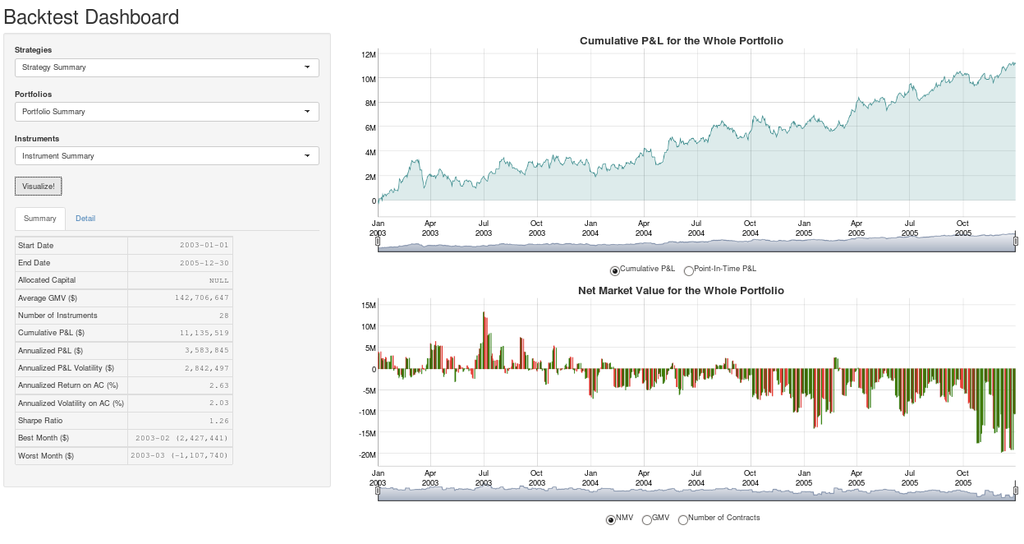
\includegraphics[width = \textwidth, height = 2.5in]{img/overallscreen.png}
\caption{The \code{backtestGraphics} interface for the \code{commodity} data frame. The interface houses three dropdown menus on the top-left to toggle between Strategies, Portfolios, and Instruments. The user may click on the ``Vizualize" button to look at the summary statistics and the interactive plots. Finally, the user can also switch between plots with the radio buttons at the bottom of the plots.
}
\end{figure}
Now, let us individually examine the various components of the Shiny interface:


\subsection{Dropdown Menus}
The interface contains three dropdown menus on the top-left to toggle between different Strategies, Portfolios, and Instruments. By selecting different combinations of these menus, the user can visualize different subsets of strategies, portfolios and instruments.


\noindent
If the given data frame does not have a \code{strategy} column, or a \code{portfolio} column, the respective dropdown menus will be fixed to ``Strategy Summary" and ``Portfolio Summary". If the user selects a combination that is incompatible with the given data frame, the interface will generate an error message and prompt the user to select a different combination.

\noindent
Figure 2 provides a screenshot of the interface's dropdown menus.

\begin{figure}[H]
\centering
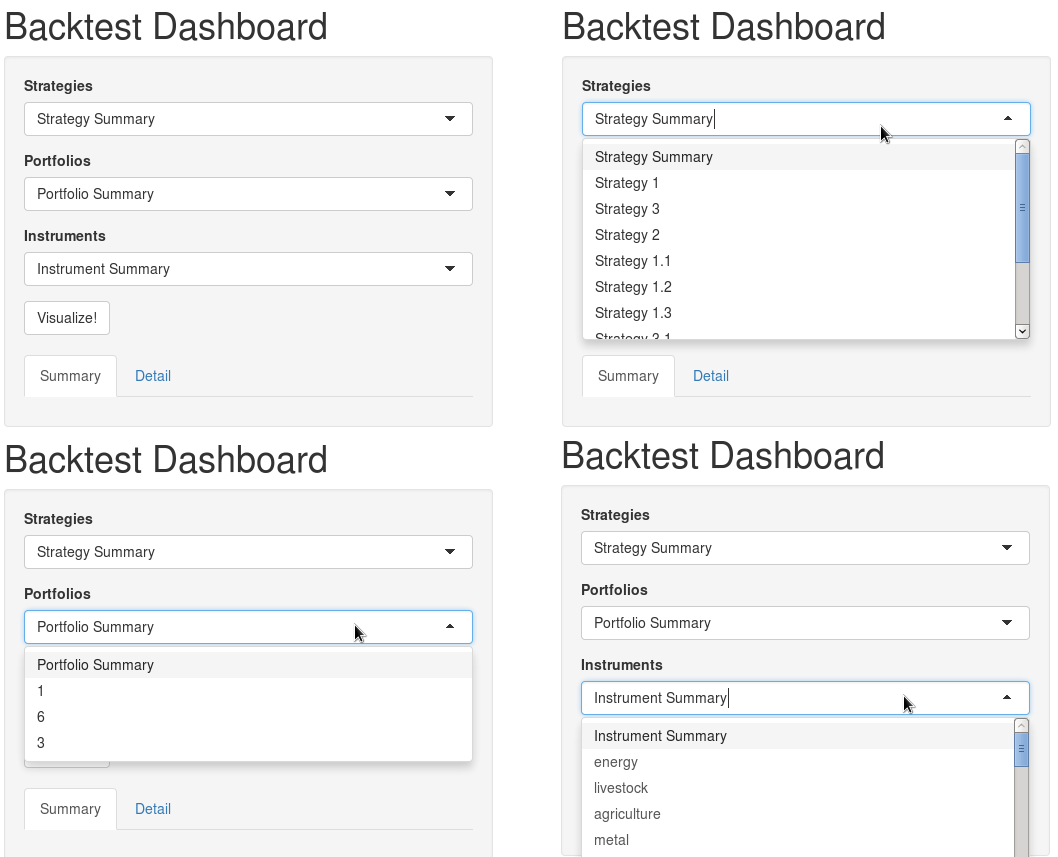
\includegraphics[width = \textwidth, height = 3in]{img/dropdown.png}
\caption{Dropdown menus: The user can subset her backtest results along different strategies, portfolios and instruments by selecting appropriate choices from the dropdown menus.}
\end{figure}

\subsection{The ``Summary" Tab}

The ``Summary" tab is present in the left-panel of the \code{Shiny} interface. It provides summary statistics for the backtest result. Figure 3 contains a screenshot of the ``Summary" tab for our commodity data frame, along with corresponding documentation.


\begin{figure}[H]
\centering
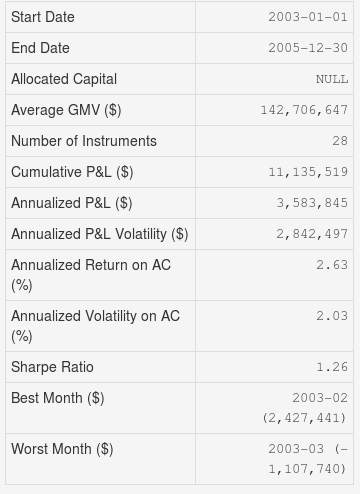
\includegraphics[width = 3in, height = 4in]{img/summary.png}
\caption{The ``Summary" tab for the \code{commodity} data frame. On clicking the ``Visualize" button, the function slices the data frame according to inputs in the drop down menus to calculate summary statistics for the specified data subset.
}
\end{figure}

Documentation of summary statistics:

\begin{itemize}
\item{Start and End date : The backtest period.}
\item{Allocated Capital : The amount of capital allocated to the portfolio. We use this number to calculate return on allocated capital. If the user does not specify this value, the corresponding entry will be \code{NULL} and `backtestGraphics` will use the highest GMV to calculate return on allocated capital.
}
\item{Average GMV : Average GMV of the portfolio over the backtest period. GMV is calculated by taking the absolute value of NMV of each instrument. }
\item{Number of Instruments : The number of different instruments in the given subset of the data frame.}
\item{Cumulative P\&L : Sum of all P\&L over the backtest period.}
\item{Annualized P\&L : This is calculated as the Average P\&L times an annualization factor. Our package observes the date interval between observations in the data frame to determine the trading frequency. The assumed annualization factor of
daily trading is $\sqrt{252}$, while that for other trading frequency is $\sqrt{\frac{365}{date \ gap}}$.}
\item{Annualized P\&L volatility : The standard deviation of all
annualized P\&L's.}
\item{Annualzied Return : Annualized average return on allocated
capital. We calculate average return rates by dividing P\&L by the allocated capital amount.  The average return rates are then annualized by multiplying them with the annualization factor.
}
\item{Sharpe Ratio : A measure of risk-adjusted return. We calculate this by dividing the mean P\&L by the standard deviation of P\&L. We assume that $\text{risk-free rate} = 0$.}
\item{Best Month and Worst Month : The month with the highest P\&L, and
the month with the lowest P\&L}
\end{itemize}

\subsubsection{The ``Detail" Tab}
The ``Detail" tab is also present in the left-panel of the \code{Shiny} interface. It provides information about the best and worst performers, as well as the biggest drawdowns. Figure 4 displays a screenshot of the ``Detail" tab for our \code{commodity} data frame, along with corresponding documentation.


\begin{figure}[H]
\centering
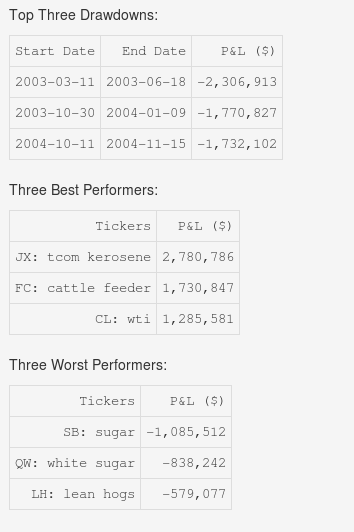
\includegraphics[width = 2.5in, height = 3.5in]{img/detail.png}
\caption{``Detail" tab with the \code{commodity} data frame.
}
\end{figure}

\noindent

Documentation of detailed statistics:

\begin{itemize}
\item{Top three drawdowns : The three biggest declines in P\&L from peak to trough. The table contains the start and end dates of the drawdowns, along with the actual value of the drawdowns.
}
\item{Best and worst three performers : The three best performers are the instruments with the highest three cumulative P\&L's. Similarly, the three worst performers are the instruments with the lowest three cumulative P\&L's. (Note: even if the user is looking at a subset of individual instruments, we will display information about the best and worst performers across all instruments. However, if the user is looking at data from a specific sector, we will display information about the best and worst performers in the specified sector).
}
\end{itemize}

\subsection{Plots}

The right-panel of our \code{Shiny} interface provides interactive plots for cumulative and point-in-time P\&L, NMV, GMV and number of contracts.

\noindent
Figure 5 provides a screenshot of the plots.

\begin{figure}[H]
\centering
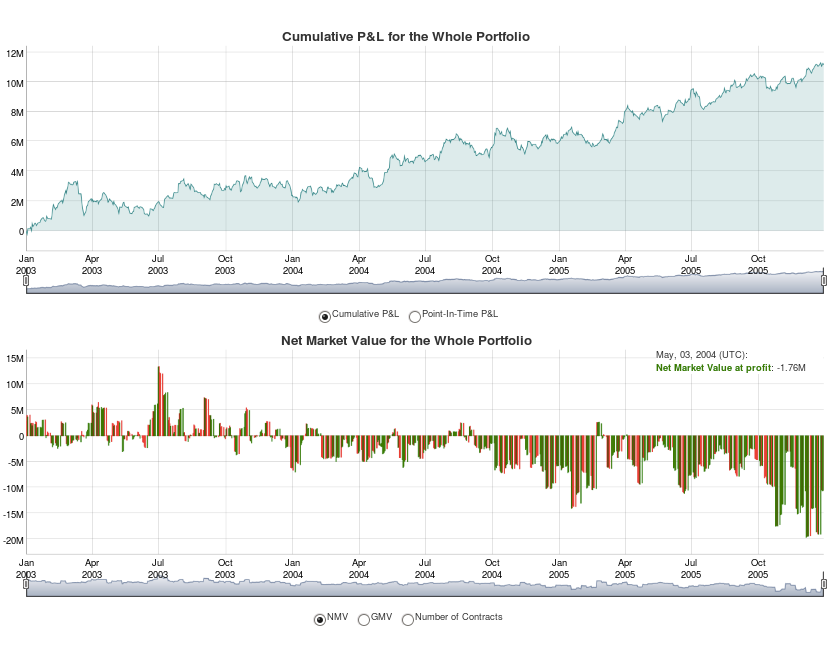
\includegraphics[width = 4in, height = 3in]{img/plots.png}
\caption{A screenshot of the plots with the \code{commodity} data frame. The P\&L plots is displayed on the top, while the market value plots are on the bottom. Radio buttons at the bottom of the plots allow the user to seamlessly switch between plots.
}
\end{figure}

\noindent
We have made the plots interactive using the \pkg{dygraphs} package [\cite{dygraphs}]. The user can zoom in to a specific time periods in a plot by dragging the corresponding region with the mouse, or changing the time slider bar, which is located below the plots. To go back to the original time scale, the user can merely double click on the respective plot. Additionally, by hovering the mouse over the plot, the user can get specific values of the response variable of the plot, on the specific date. The color of the plots is based on the sign of the point-in-time P\&L. Green bars represent profits, while the red bars represent losses.





%% -- Summary/conclusions/discussion -------------------------------------------

\section{Conclusion} \label{sec:conclusion}

The \pkg{backtestGraphics} package provides a simple \code{Shiny} interface to visualize backtest results. Inside the package, we have provided three sample data frames. The user can use the code provided in this document to test the package with these data frames. 


\noindent
Our interface provides the user with summary, as well as detailed statistics about the backtest result. The user can subset her data according to strategies, sub-strategies, and instruments. Additionally, we also provide interactive plots that show movement of important variables over the backtest period. 


\noindent
These are powerful tools to uncover trends and anomalies in the data. By decomposing the data frame into different sectors and instruments, the user can gain important insights into his trading strategies over different sectors and time periods. The interactive plots provide additional flexibility to dive into the nitty-gritty details of the backtest.

\noindent
Going forward, the \pkg{backtestGraphics} package can easily be customized to suit the needs of a specific user. Such customization may include, among others, adding new response variables to plots, redesigning plots, or introducing additional summary statistics. We invite users to take advantage of this, and redesign the \pkg{backtestGraphics} interface according to their preferences. 



%% -- Bibliography -------------------------------------------------------------
%% - References need to be provided in a .bib BibTeX database.
%% - All references should be made with \cite, \citet, \citep, \citealp etc.
%%   (and never hard-coded). See the FAQ for details.
%% - JSS-specific markup (\proglang, \pkg, \code) should be used in the .bib.
%% - Titles in the .bib should be in title case.
%% - DOIs should be included where available.

\bibliography{backtestGraphics}


%% -- Appendix (if any) --------------------------------------------------------
%% - After the bibliography with page break.
%% - With proper section titles and _not_ just "Appendix".



%% -----------------------------------------------------------------------------


\end{document}
